\documentclass[landscape,a4paper,12pt,french, twocolumn]{article}

\usepackage{../../Style}

\begin{document}

\title{\vspace{-1cm} Vecteurs du plan: Première approche \vspace{-1cm} }
\author{}
\date{}
\maketitle

\begin{FlushLeft}

\rem{Voir activité d'introduction}

\section{Translations}

Soient $A,B,M$ trois points quelconques du plan. L'image de $M$ par la translation de vecteur $\vv {AB}$ est l'unique point $N$ tel que le quadrilatère $ABNM$ soit un parallélogramme.

\begin{center}
\begin{tikzpicture}[scale=0.7]
\node[color=black,circle,minimum size=1pt,fill,inner sep=2pt,label={90:\textbf{\large A}}] (A) at (0,0) {};
\node[color=black,circle,minimum size=1pt,fill,inner sep=2pt,label={90:\textbf{\large B}}] (B) at (5,-2) {};
\node[color=black,circle,minimum size=1pt,fill,inner sep=2pt,label={90:\textbf{\large M}}] (M) at (-2,-3) {};
\node[color=red,circle,minimum size=1pt,fill,inner sep=2pt,label={90:\textbf{\large \color{red} N}}] (N) at (3,-5) {};
\draw[color=red,thick, -] (M) +(-17:5.385) arc (-17:-27:5.385);
\draw[color=red,thick, -] (B) +(-115:3.606) arc (-115:-132:3.606);
%\draw[dashed] (M) circle (5.3851);
%\draw (B) circle (3.6055);

\end{tikzpicture}
\end{center}

\begin{rmqs}
Lors de cette translation:
\begin{itemize}
\item Les droites $(AB)$ et $(MN)$ sont parallèles
\item Les longueurs $AB$ et $MN$ sont égales
%\item Le glissement de $M$ vers $N$ se fait dans la même sens que de $A$ vers $B$.
\end{itemize}
\end{rmqs}

\section{Généralités sur les vecteurs}

Un vecteur $\vec u$ peut être représenté avec une origine $A$ et une extrémité $B$. Il est caractérisé par:
\begin{itemize}
\item Sa direction ( celle de la droite $(AB)$ )
\item Son sens ( de $A$ vers $B$ )
\item Sa norme ( ou sa longueur ), notée $\Vert \vec u \Vert$. On a $\Vert \vec u \Vert = AB$.
\end{itemize}

\textbf{Egalité de deux vecteurs:}
Lorsque deux vecteurs symbolisent le même déplacement, on dit qu'ils sont égaux. La figure précédente nous donne alors $\vv{AB} = \vv {MN}, \vv{BA} = \vv{NM}, \vv {AM} = \vv {BN}$.

\begin{propr}
Les quatre propositions suivantes sont \textbf{équivalentes}:
\begin{itemize}
\item $\vv {AB} = \vv {MN}$
\item $N$ est l'image de $M$ par la translation de vecteur $\vv{AB}$
\item $[AN]$ et $[BM]$ se coupent en leur milieu
\item $ABNM$ est un parallélogramme
\end{itemize}
\end{propr}

\textbf{Quelques exemples particuliers:}
\begin{itemize}
\item Le vecteur nul, noté $\vv 0$, est obtenu à partir de la translation qui transforme $A$ et $A$, $B$ en $B$ ... On a alors $\vv 0 = \vv {AA} = \vv {BB} = \ldots$ Ce vecteur n'a ni direction, ni sens, et sa norme est nulle.
\item L'opposé du vecteur $\vv {AB}$ est le vecteur associé à la translation qui transforme $B$ en $A$. On le note $- \vv {AB}$. Ainsi, $- \vv {AB} = \vv {BA}$. Il a la même direction et la même norme que $\vv {AB}$ mais est de sens contraire.
\end{itemize}

\section{Somme de deux vecteurs}

\rem{Voir activité somme de deux vecteurs}

\begin{center}
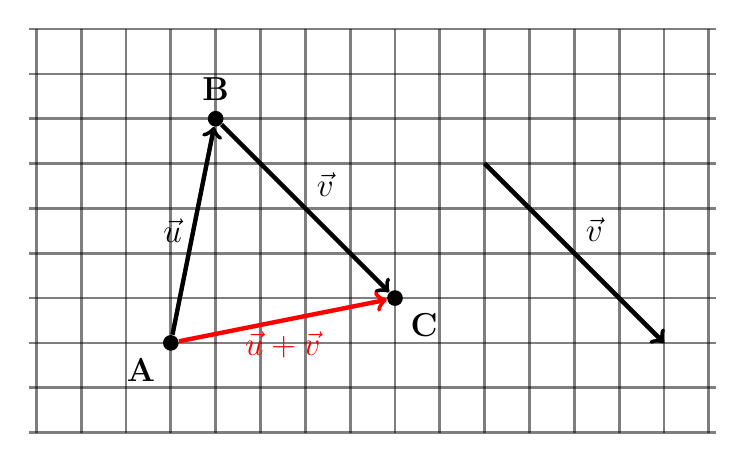
\begin{tikzpicture}
\begin{axis}[
%axis x line=bottom,
%axis y line = left,
%axis lines=middle,
width=0.93\linewidth,
height=0.6\linewidth,
xmin=0, xmax=13,
ymin=0, ymax=9,
%enlargelimits={abs=0.2},
xtick distance=1,
ytick distance=1,
grid=both,
xticklabels={},
yticklabels={},
grid style={black,line width=1pt, draw opacity=0.5},
ticks=none,
axis equal,
legend pos=north east,
axis line style={draw=none},
scale=0.9
]
\node[color=black,circle,minimum size=1pt,fill,inner sep=2pt,fill opacity=1,label={-135:\textbf{\large A}}] (A) at (2,2) {};
\node[color=black,circle,minimum size=1pt,fill,inner sep=2pt,fill opacity=1,label={90:\textbf{\large B}}] (B) at (3,7) {};
\draw[ultra thick,->] (A) -- (B) node[pos=0.5,left] {\large $\vec u$};
\draw[ultra thick,->] (9,6) -- (13,2) node[pos=0.5,above right] {\large $\vec v$};
\node[color=black,circle,minimum size=1pt,fill,inner sep=2pt,fill opacity=1,label={-45:\textbf{\large C}}] (C) at (7,3) {};
\draw[ultra thick,->] (B) -- (C) node[pos=0.5,above right] {\large $\vec v$};
\draw[ultra thick,->,color=red] (A) -- (C) node[pos=0.5,below] {\large $\vec u + \vec v$};

\end{axis}
\end{tikzpicture}
\end{center}

\begin{ex}
$\vv {AB} + \vv {BA} = \vv {AA} = \vv 0$
\end{ex}

\textbf{Attention :} En général, la longueur de $\vec u + \vec v$ n'est pas égale à la somme de celle de $\vec u$ et de $\vec v$: $\Vert \vec u + \vec v \Vert \neq \Vert \vec u \Vert + \Vert \vec v \Vert$

\textbf{Méthode :} Pour construire $\vv {AB} + \vv {AC}$, il suffit de construire le parallélogramme $ABDC$ et de prendre le vecteur $\vv {AD}$.

\begin{center}
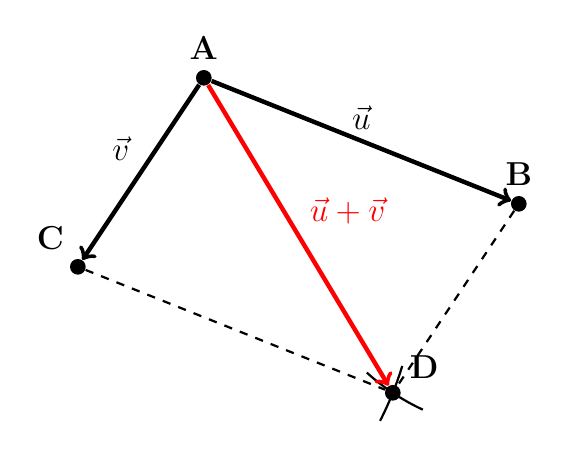
\begin{tikzpicture}[scale=0.8]

\node[color=black,circle,minimum size=1pt,fill,inner sep=2pt,label={90:\textbf{\large A}}] (A) at (0,0) {};
\node[color=black,circle,minimum size=1pt,fill,inner sep=2pt,label={90:\textbf{\large B}}] (B) at (5,-2) {};
\node[color=black,circle,minimum size=1pt,fill,inner sep=2pt,label={120:\textbf{\large C}}] (C) at (-2,-3) {};
\node[color=black,circle,minimum size=1pt,fill,inner sep=2pt,label={30:\textbf{\large D}}] (D) at (3,-5) {};
\draw[thick, -] (C) +(-17:5.385) arc (-17:-27:5.385);
\draw[thick, -] (B) +(-115:3.606) arc (-115:-132:3.606);
\draw[ultra thick,->] (A) -- (B) node[pos=0.5,above] {\large $\vec u$};
\draw[ultra thick,->] (A) -- (C) node[pos=0.5,above left] {\large $\vec v$};
\draw[color=red,ultra thick,->] (A) -- (D) node[pos=0.5,above right] {\large $\vec u + \vec v$};
\draw[dashed,thick,-] (B) -- (D);
\draw[dashed,thick,-] (C) -- (D);

\end{tikzpicture}
\end{center}

\section{Produit d'un vecteur par un nombre réel}

Soit $k$ un réel et $\vec u$ un vecteur. Le produit de $k$ par $\vec u$ est le vecteur noté $k \vec u$ tel que:
\begin{itemize}
\item $\vec u$ et $k \vec u$ ont la même direction
\item La longueur de $k \vec u$ est $\abs k \Vert \vec u \Vert$
\item Si $k > 0$, $\vec u$ et $k \vec u$ ont le même sens. Sinon, ils ont des sens opposés.
\end{itemize}

\begin{rmq}
En particulier, $0 \times \vec u = \vv 0$.
\end{rmq}

\begin{ex} \

\begin{center}
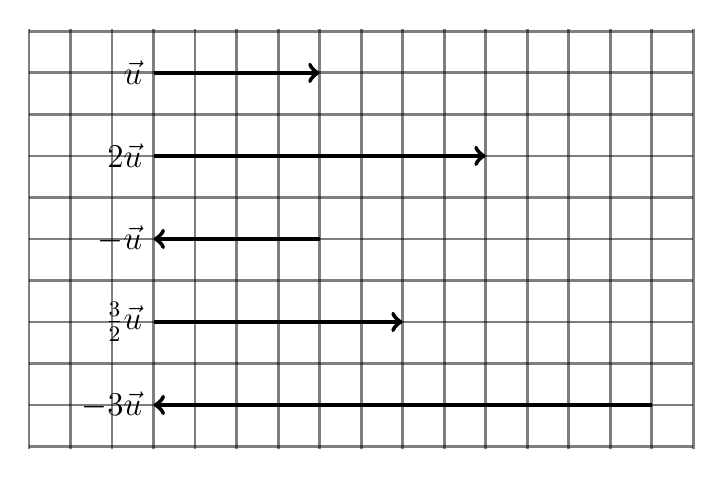
\begin{tikzpicture}[scale=1]
\begin{axis}[
%axis x line=bottom,
%axis y line = left,
%axis lines=middle,
width=\linewidth,
height=0.68\linewidth,
xmin=-3, xmax=13,
ymin=-9, ymax=1,
%enlargelimits={abs=0.2},
xtick distance=1,
ytick distance=1,
grid=both,
xticklabels={},
yticklabels={},
grid style={black,line width=1pt, draw opacity=0.5},
ticks=none,
axis equal,
legend pos=north east,
axis line style={draw=none},
scale=0.8
]


\draw[ultra thick,->] (0,0) -- (4,0) node[pos=0,left] {\large $\vec u$};
\draw[ultra thick,->] (0,-2) -- (8,-2) node[pos=0,left] {\large $2 \vec u$};
\draw[ultra thick,<-] (0,-4) -- (4,-4) node[pos=0,left] {\large $-\vec u$};
\draw[ultra thick,->] (0,-6) -- (6,-6) node[pos=0,left] {\large $\frac 3 2 \vec u$};
\draw[ultra thick,<-] (0,-8) -- (12,-8) node[pos=0,left] {\large $-3\vec u$};

\end{axis}
\end{tikzpicture}
\end{center}

\end{ex}

\begin{app}
$I$ est le milieu de $[AB]$ se traduit par $\vv {AI} = \vv {IB}$ ou $\vv{AB} = 2\vv{AI}$ ou $\vv {AI} = \frac 1 2 \vv{AB}$.
\end{app}

\begin{center}
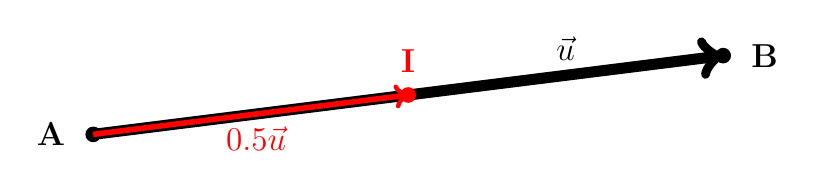
\begin{tikzpicture}
\draw[line width=4pt,->] (0,0) -- (8,1) node[pos=0.75,above] {\large $\vec u$} node[pos=0,color=black,circle,minimum size=1pt,fill,inner sep=2pt,label={180:\textbf{\large A}}] {} node[pos=1,color=black,circle,minimum size=1pt,fill,inner sep=2pt,label={0:\textbf{\large B}}] {};
\draw[line width=2pt, color=red, ->] (0,0) -- (4,0.5) node[pos=0.5,below] {\large { $0.5\vec u$} } node[pos=1,color=red,circle,minimum size=1pt,fill,inner sep=2pt,label={90:\textbf{\large I}}] {};
\end{tikzpicture}
\end{center}

\end{FlushLeft}

\end{document}
